\section{Předpřipravené ukázky}

Pokud je váš počítač chráněný firewallem nebo proxy serverem, zkontrolujte, že má Firefox povolený přístup k internetu.
\todo{Todo section}

\subsection{Pseudokod algoritmu}

\begin{algorithm}[h]
\For{$i = 0$ \KwTo $100$}{
 print\_number = true\;
\If{i is divisible by 3}{
 print\_number = false\;
}
\If{i is divisible by 5}{
 print "Buzz"\;
}
print a newline\;
}
\caption{Ukázka pseudokodu algoritmu}
\end{algorithm}

\subsection{Kod v programovacím jazyce}

\begin{lstlisting}[caption = Print arguments of command line]
#include <stdio.h>

/**
 * Comments are gray but it can by styled by configure values in dokumentace.tex
 *
 * @param int argc Count of arguments of command line
 * @param *char[] argv List of command line arguments
 */
int main(int argc, char *argv[]) {
	
	// For cycle
    for(int i = 0; i < argc; i++) {
    	printf("%s\n", argv[i]);
    }
    return 0;
}
\end{lstlisting}
\subsection{Vizualizace datových struktur}
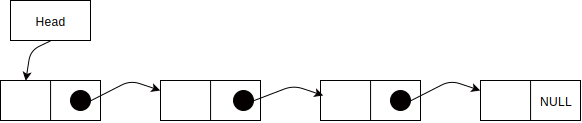
\includegraphics{./build/data_structure.pdf}